% ─────────────────────────────────────────────────────────────────────
%  Capítulo 8 — Marco regulador y entorno socioeconómico
% ─────────────────────────────────────────────────────────────────────
\chapter{Marco regulador y entorno socioeconómico}
\label{cap:regulador}

Un sistema como el descrito en este TFG no puede entenderse al margen del marco normativo en el que tendría que vivir en producción. Este capítulo recorre las normas aplicables a un detector FDI desplegado sobre infraestructura de medida avanzada en España y la Unión Europea, y completa la fotografía con el entorno socioeconómico del proyecto: presupuesto, planificación e impacto.

\section{Marco regulador}
\label{sec:regulador}

Cualquier despliegue real de este sistema tendría que convivir con varias capas normativas que se solapan: protección de datos, ciberseguridad de infraestructuras críticas, regulación sectorial del eléctrico y normas técnicas específicas. Las repasamos a continuación, una por una.

\subsection{Protección de datos personales}

\paragraph{Reglamento General de Protección de Datos.} El RGPD ---formalmente Reglamento (UE) 2016/679 \cite{rgpd2016}--- es el marco europeo de protección de datos personales y aplica de pleno a este caso. Los datos de consumo eléctrico de un hogar son, sin lugar a dudas, datos personales: revelan hábitos de vida (presencia, ausencia, horarios), uso de electrodomésticos concretos y, agregados en el tiempo, perfiles sociodemográficos identificables \cite{molina2010private}.

Los principios del artículo 5 son los que tienen tracción directa. La licitud del tratamiento se sostiene sobre la ejecución del contrato de suministro y el interés legítimo en prevenir el fraude. La minimización exige quedarse con lo estrictamente necesario ---en nuestro caso, las medidas eléctricas estándar---, y la limitación de la finalidad impide derivar la detección de FDI hacia perfiles comerciales sin consentimiento explícito del usuario. A todo ello se añaden la exactitud y la conservación limitada de los datos.

\paragraph{LOPDGDD.} La Ley Orgánica 3/2018 \cite{lopdgdd2018}, de Protección de Datos Personales y Garantía de los Derechos Digitales, trae el RGPD al ordenamiento español y añade algunas especificaciones nacionales. La que más conviene tener presente aquí es el artículo 22, sobre decisiones automatizadas: el sujeto tiene derecho a no ser objeto de decisiones basadas únicamente en tratamiento automatizado que produzcan efectos jurídicos sobre él. Una alarma de FDI, por sí sola, no produce efectos jurídicos directos ---la sanción o la investigación requieren un proceso humano posterior---, pero el operador sigue obligado a informar al sujeto del tratamiento y a darle vías de oposición efectivas.

\paragraph{Implicaciones prácticas para el sistema.} El despliegue \textit{edge} encaja particularmente bien con el RGPD por una razón directa: el dato sensible no sale del contador, sólo las alarmas viajan al concentrador. Eso constituye una minimización por diseño, lo que reduce la exposición y simplifica el cumplimiento. A esta arquitectura conviene añadirle dos prácticas habituales. Por un lado, pseudonimizar el identificador del contador en cualquier entorno de investigación o agregación, de modo que el conjunto de muestras no permita re-identificar al usuario. Por otro, garantizar los derechos del interesado: la distribuidora debe informar de la existencia del detector y del tratamiento asociado, y proporcionar vías de acceso, rectificación y oposición. Finalmente, un despliegue masivo de este tipo sobre infraestructura crítica encaja en el supuesto de \textit{Data Protection Impact Assessment} del artículo 35 del RGPD, y por tanto exige una DPIA previa.

\paragraph{Privacidad por diseño: federated learning y privacidad diferencial.} La arquitectura \textit{edge} satisface la minimización del artículo 5, pero el \emph{entrenamiento} del detector sigue siendo un punto sensible si exige reunir series de consumo de muchos hogares. La ampliación de este trabajo (\cref{sec:resultados-ampliacion}) materializa la \textbf{privacidad por diseño} del artículo 25 con dos mecanismos concretos: el \emph{federated learning} (FedAvg) entrena un modelo compartido \emph{sin} que los datos crudos abandonen el contador ---solo se intercambian pesos---, y la \emph{privacidad diferencial} (DP-SGD) añade una garantía matemática $(\varepsilon,\delta)$ que acota formalmente cuánto puede inferir un adversario sobre un hogar individual a partir del modelo entrenado, mitigando los ataques de inferencia de pertenencia. El presupuesto $\varepsilon$ se convierte así en un parámetro auditable de cumplimiento: cuanto menor, mayor la protección del interesado. Esta combinación es directamente relevante para un despliegue a escala nacional (decenas de millones de contadores) sin centralización de datos personales.

\subsection{Ciberseguridad de infraestructuras críticas}

\paragraph{Directiva NIS2.} La NIS2 ---Directiva (UE) 2022/2555 \cite{nis2directive}, aplicable en España desde enero de 2024--- sustituye y refuerza a la NIS de 2016, y cubre operadores de servicios esenciales, entre ellos el sector energético. Las obligaciones que introduce se pueden resumir en tres frentes: gestión de riesgos (políticas de seguridad, análisis de riesgo y controles técnicos y organizativos), notificación de incidentes a la autoridad nacional ---con plazos estrictos: alerta inicial en 24 horas e informe detallado en 72 horas--- y responsabilidad sobre la cadena de suministro, en virtud de la cual el operador responde también por la seguridad de sus proveedores.

Un detector FDI desplegado encaja directamente en el primer frente: es un control técnico más dentro de la gestión de riesgos del operador. Pero hay una segunda implicación menos evidente: los incidentes que detecta el sistema pueden activar la obligación de notificación, lo que se traduce en requisitos operativos sobre la calidad de la detección y, sobre todo, sobre el número aceptable de falsos positivos.

\paragraph{Ley 8/2011 PIC.} La Ley 8/2011 \cite{ley8_2011_pic}, de protección de infraestructuras críticas, define el sector energético como crítico y establece el régimen de protección. El \textit{Centro Nacional de Protección de Infraestructuras y Ciberseguridad} (CNPIC) coordina la protección a nivel nacional. El \emph{Plan Estratégico Sectorial} de la energía y los \emph{Planes de Protección Específicos} de los operadores recogen las medidas concretas.

\paragraph{INCIBE-CERT.} El \emph{Instituto Nacional de Ciberseguridad} opera el \emph{CERT} (\textit{Computer Emergency Response Team}) de referencia para incidentes en operadores no críticos y, junto con el CNPIC, coordina la respuesta sectorial. Un detector FDI puede integrarse en los procesos de \emph{threat intelligence} compartida con INCIBE-CERT.

\subsection{Regulación del sector eléctrico}

\paragraph{Directivas europeas de eficiencia y mercado interior.} La Directiva 2009/72/CE y sus sucesoras (2018/2001, 2019/944) impulsaron el despliegue de contadores inteligentes en la Unión Europea con el objetivo de cubrir al menos el 80\% de los consumidores. La directiva 2018/2001 \cite{red_iii} (\emph{REDII}) refuerza el papel del consumidor activo (autoconsumo, agregación), que requiere medición fiable como condición previa.

\paragraph{Marco español de telegestión.} La Orden ITC/3860/2007 \cite{itc3860} estableció el plan español de sustitución de contadores tradicionales por contadores inteligentes con telegestión, completado en 2018--2019. Las especificaciones técnicas (PRIME, PLC G3, IEC 14908) regulan la comunicación entre contador y concentrador.

\paragraph{Tarifas y sanciones.} El régimen sancionador por fraude eléctrico está en la Ley 24/2013 del Sector Eléctrico \cite{ley24_2013} y en el Real Decreto 1955/2000 sobre actividad de transporte, distribución y suministro. Las distribuidoras pueden recuperar el consumo defraudado, aplicar penalizaciones y proceder al corte del suministro tras procedimiento.

\subsection{Normas técnicas}

\paragraph{IEC 62351.} La serie IEC 62351 \cite{iec62351} es la norma técnica de referencia en ciberseguridad para \textit{smart grids}. Cubre autenticación de comunicaciones, cifrado, integridad, control de acceso, gestión de claves y operación segura sobre los protocolos SCADA (IEC 60870-5, IEC 61850, DNP3). Aquí conviene matizar bien: un sistema FDI bien diseñado debe asumir que el protocolo ya está cifrado y autenticado conforme a IEC 62351, y aún así seguir detectando ataques. La razón es directa: la criptografía protege el dato en tránsito pero no defiende del compromiso de los \textit{endpoints}, y un atacante con acceso al contador puede firmar lecturas falsas de forma perfectamente legítima.

\paragraph{ISO/IEC 27001 y 27002.} El sistema de gestión de seguridad de la información (SGSI) ISO/IEC 27001 \cite{iso27001} y los controles ISO/IEC 27002 son el marco generalista de aplicación. Aspectos relevantes para un detector FDI: gestión de incidentes (A.16), seguridad en las comunicaciones (A.13), cifrado (A.10), y registro y monitorización (A.12).

\paragraph{NIST Cybersecurity Framework.} El \emph{NIST Cybersecurity Framework} v1.1 \cite{nist_csf} y la guía NIST SP 800-82 \cite{nist80082} para sistemas industriales y de control proporcionan un marco de referencia complementario, especialmente influyente en operadores con presencia internacional.

\subsection{Propiedad intelectual}

\paragraph{Licencia del dataset UCI.} El \emph{Individual Household Electric Power Consumption} se distribuye bajo licencia \emph{Creative Commons Attribution 4.0 International} (CC BY 4.0), que permite el uso, redistribución y modificación con atribución. La autoría se reconoce explícitamente en la bibliografía \cite{hebrail2012uci}.

\paragraph{Licencias del software.} El software utilizado es íntegramente \emph{open source} con licencias permisivas:
\begin{itemize}[leftmargin=*,topsep=0pt]
  \item TensorFlow / Keras: Apache License 2.0.
  \item scikit-learn: BSD-3-Clause.
  \item LightGBM: MIT.
  \item Python: PSF License.
  \item NumPy, pandas, matplotlib, SHAP: BSD-3-Clause.
\end{itemize}
Todas son compatibles entre sí y permiten uso comercial. El TFG se publica bajo CC BY-NC-SA 4.0; el código del repositorio está bajo MIT.

\section{Entorno socioeconómico}
\label{sec:socioeconomico}

\subsection{Impacto económico del problema}

Las cifras del problema son grandes en cualquier dirección que se las mire. A nivel global, las pérdidas no técnicas (NTL) rondan el 1--3\,\% de la energía distribuida en países desarrollados y llegan al 30--40\,\% en algunas economías emergentes \cite{messinis2018review,viegas2017review}, lo que se traduce en más de 96\,000 millones de dólares anuales en todo el mundo. En España, según la CNMC, las distribuidoras estiman entre 7\,000 y 9\,000\,GWh al año de NTL ---en torno al 2--3\,\% del consumo facturado---, con un coste agregado que acaba trasladándose al consumidor final vía peajes.

Sobre esa base, un sistema de detección automática que recuperase incluso un 10--20\,\% de esas pérdidas tendría un impacto anual del orden de centenares de millones de euros sólo en España, y eso sin contar el efecto disuasorio sobre el fraude organizado ---cultivos ilícitos, minería de criptomonedas no declarada y similares. El coste de despliegue del sistema propuesto, además, es marginal: el hardware ya existe (los contadores inteligentes están instalados), y lo único que se requiere es desplegar el software adicional.

\subsection{Presupuesto del TFG}

\begin{table}[H]
\centering
\caption{Presupuesto del proyecto.}
\label{tab:presupuesto}
\small
\begin{tabularx}{\textwidth}{X r r r}
\toprule
Concepto & Unidades & Coste unitario & Total \\
\midrule
Personal & & & \\
\quad Estudiante (TFG)         & 400\,h    & 15\,\euro/h & 6000\,\euro \\
\quad Tutor/a (dirección)      & 30\,h     & 50\,\euro/h & 1500\,\euro \\
\midrule
Hardware (amortización 4 años) & & & \\
\quad MacBook M2 Pro 16\,GB    & 6 meses   & 2500\,\euro\,/\,48\,m & 313\,\euro \\
\quad Disco externo 1\,TB      & 6 meses   & 200\,\euro\,/\,48\,m  & 25\,\euro \\
\midrule
Software / Servicios & & & \\
\quad Sistema operativo (macOS)         & ---       & gratuito     & 0\,\euro \\
\quad Python, TF, scikit-learn, LightGBM & ---       & FOSS         & 0\,\euro \\
\quad Servicios cloud (descartado)      & ---       & ---          & 0\,\euro \\
\midrule
Otros & & & \\
\quad Bibliografía y revistas (acceso UC3M)        & ---       & ---       & 0\,\euro \\
\quad Impresión y encuadernación (5 ejemplares)    & 5         & 25\,\euro   & 125\,\euro \\
\midrule
Costes indirectos (15\%)        &           &              & 1194\,\euro \\
\midrule
\textbf{Total}                  &           &              & \textbf{9157\,\euro} \\
\bottomrule
\end{tabularx}
\end{table}

La práctica totalidad del coste es \emph{personal} (estudiante + tutor), lo que es consistente con la naturaleza investigadora del proyecto. El software es 100\% \emph{open source}, lo que evidencia que el sistema propuesto puede replicarse sin coste de licencias.

\subsection{Cronograma del proyecto}

El reparto temporal de las siete fases del proyecto se muestra en la \cref{fig:gantt}, sobre el calendario académico real, y se traduce a horas dedicadas en la \cref{tab:gantt}.

\begin{figure}[H]
\centering
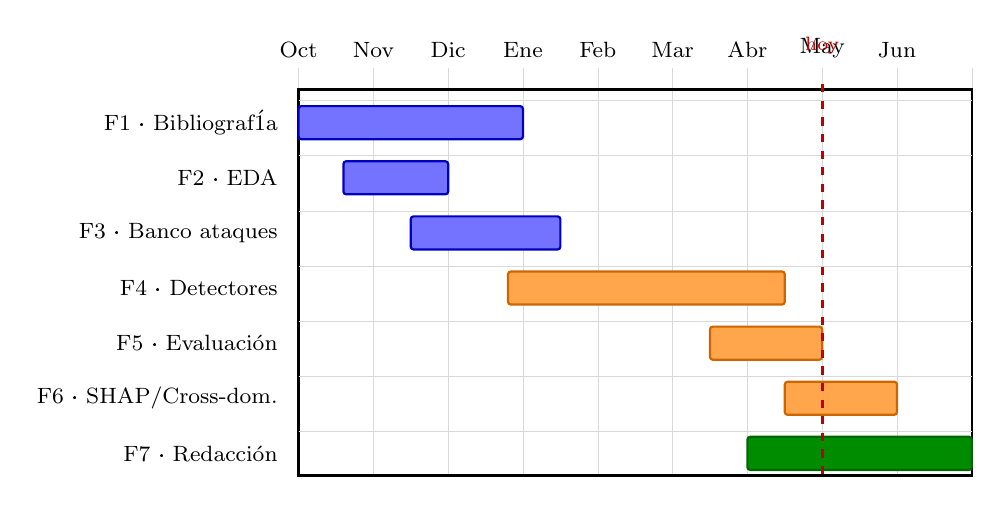
\begin{tikzpicture}[x=0.95cm, y=0.7cm,
    bar/.style={fill=blue!55, draw=blue!75!black, thick, rounded corners=1pt},
    barb/.style={fill=orange!70, draw=orange!80!black, thick, rounded corners=1pt},
    barr/.style={fill=green!55!black, draw=green!40!black, thick, rounded corners=1pt},
    grid/.style={gray!30, very thin},
    every node/.style={font=\footnotesize}]
  % Eje meses (1..10 = oct 2025 a jul 2026)
  \foreach \x/\lbl in {0/Oct, 1/Nov, 2/Dic, 3/Ene, 4/Feb, 5/Mar, 6/Abr, 7/May, 8/Jun} {
    \draw[grid] (\x,0) -- (\x,-7.4);
    \node[above] at (\x,0) {\lbl};
  }
  \draw[grid] (9,0) -- (9,-7.4);
  % Marco
  \draw[thick] (0,-0.4) rectangle (9,-7.4);
  % Filas
  \foreach \i in {1,...,7} { \draw[grid] (0,-\i*1+0.4) -- (9,-\i*1+0.4); }
  % Etiquetas de fase (eje izquierdo)
  \foreach \i/\name in {
      1/{F1 · Bibliografía},
      2/{F2 · EDA},
      3/{F3 · Banco ataques},
      4/{F4 · Detectores},
      5/{F5 · Evaluación},
      6/{F6 · SHAP/Cross-dom.},
      7/{F7 · Redacción}}{
    \node[anchor=east] at (-0.15,-\i+0.0) {\name};
  }
  % Barras (x_inicio, x_fin) en meses desde Oct
  \draw[bar]  (0.0,-1.3) rectangle (3.0,-0.7);   % F1 Bibliografía  oct-ene
  \draw[bar]  (0.6,-2.3) rectangle (2.0,-1.7);   % F2 EDA           nov-dic
  \draw[bar]  (1.5,-3.3) rectangle (3.5,-2.7);   % F3 Ataques       dic-feb
  \draw[barb] (2.8,-4.3) rectangle (6.5,-3.7);   % F4 Detectores    feb-may
  \draw[barb] (5.5,-5.3) rectangle (7.0,-4.7);   % F5 Evaluación    abr-may
  \draw[barb] (6.5,-6.3) rectangle (8.0,-5.7);   % F6 SHAP/CD       may-jun
  \draw[barr] (6.0,-7.3) rectangle (9.0,-6.7);   % F7 Redacción     may-jul
  % Línea hoy (mayo 2026 = x=7)
  \draw[red!75!black, very thick, dashed] (7,-0.3) -- (7,-7.5);
  \node[red!75!black, font=\scriptsize] at (7,0.4) {hoy};
\end{tikzpicture}
\caption{Cronograma del proyecto. Azul: revisión y diseño. Naranja: implementación y evaluación. Verde: redacción. La línea roja discontinua marca el momento actual.}
\label{fig:gantt}
\end{figure}

\begin{table}[H]
\centering
\caption{Fases del proyecto y horas dedicadas.}
\label{tab:gantt}
\small
\begin{tabularx}{\textwidth}{l X r}
\toprule
Fase & Descripción & Horas \\
\midrule
1 & Revisión bibliográfica y estado del arte & 50 \\
2 & Análisis exploratorio del dataset UCI    & 40 \\
3 & Diseño e implementación del banco de ataques (NB02) & 50 \\
4 & Implementación de detectores (NB03--NB10)           & 130 \\
5 & Evaluación, optimización, recalibración             & 60 \\
6 & Análisis adicional: SHAP, cross-domain, robustez    & 30 \\
7 & Redacción de la memoria                              & 40 \\
\midrule
\textbf{Total}  &                                                  & \textbf{400} \\
\bottomrule
\end{tabularx}
\end{table}

\subsection{Impacto social y ambiental}

\paragraph{Impacto social.} Detectar el fraude eléctrico de forma eficaz tiene un efecto redistributivo claro: a día de hoy, las pérdidas no técnicas se acaban recargando en la tarifa de todos los consumidores, también los honestos. Además, la detección automática y de bajo coste evita la \textit{ronda física} de inspección, que es invasiva para el cliente y cara para la distribuidora. Hay otra dimensión social que también pesa, la de la privacidad: un detector que vive en el \textit{edge} mantiene el dato sensible dentro del contador y sólo envía alarmas aguas arriba; es claramente preferible a una arquitectura centralizada en la nube, donde toda la información de consumo se concentra en un único punto y cualquier brecha tiene un impacto magnificado.

\paragraph{Impacto ambiental.} El consumo energético del propio detector es despreciable. Una inferencia del Dense-AE consume del orden de microjulios sobre un microcontrolador moderno, y sobre las 525\,600 inferencias anuales que supone procesar un minuto cada vez, el consumo agregado se queda en unas décimas de joule por contador y año ---unas $10^{-7}$ veces el consumo del propio hogar. El entrenamiento sí tiene un coste energético, pero también modesto: unos minutos de GPU. El despliegue, prácticamente nada. Indirectamente, además, reducir el fraude contribuye a la eficiencia del sistema eléctrico: las pérdidas no técnicas son energía generada que no se factura, lo que obliga al operador a despachar capacidad adicional para cubrirlas. Recortarlas en un 1\,\% del consumo nacional equivaldría a varias decenas de GWh anuales de generación evitada.

\paragraph{Objetivos de Desarrollo Sostenible.} El proyecto contribuye a varios ODS:
\begin{itemize}[leftmargin=*,topsep=0pt]
  \item \textbf{ODS 7} (Energía asequible y no contaminante): mejora de la eficiencia del sistema eléctrico.
  \item \textbf{ODS 9} (Industria, innovación e infraestructura): infraestructura resiliente vía detección de amenazas.
  \item \textbf{ODS 11} (Ciudades sostenibles): infraestructuras urbanas más fiables.
  \item \textbf{ODS 16} (Paz, justicia e instituciones sólidas): combate del fraude organizado vinculado a actividades ilícitas.
\end{itemize}
